\documentclass[a4paper, 12pt]{article}
\usepackage{geometry}
\usepackage{graphicx}
\usepackage{mathtools}
\usepackage{listings}
\usepackage{float}
\usepackage[utf8]{inputenc}
\geometry{margin=1in}


\begin{document}

\section{Opdrachten}

\subsection{Bij een gewenste waarde = $22^\circ$C en een buitentemperatuur = $9,5^\circ$C, treedt er verzadiging op in het stuursignaal zolang de werkelijke temperatuur $>$ $24^\circ$C of kleiner dan $20^\circ$C. \\ Verifieer en verklaar!}

\begin{figure}[!h]
	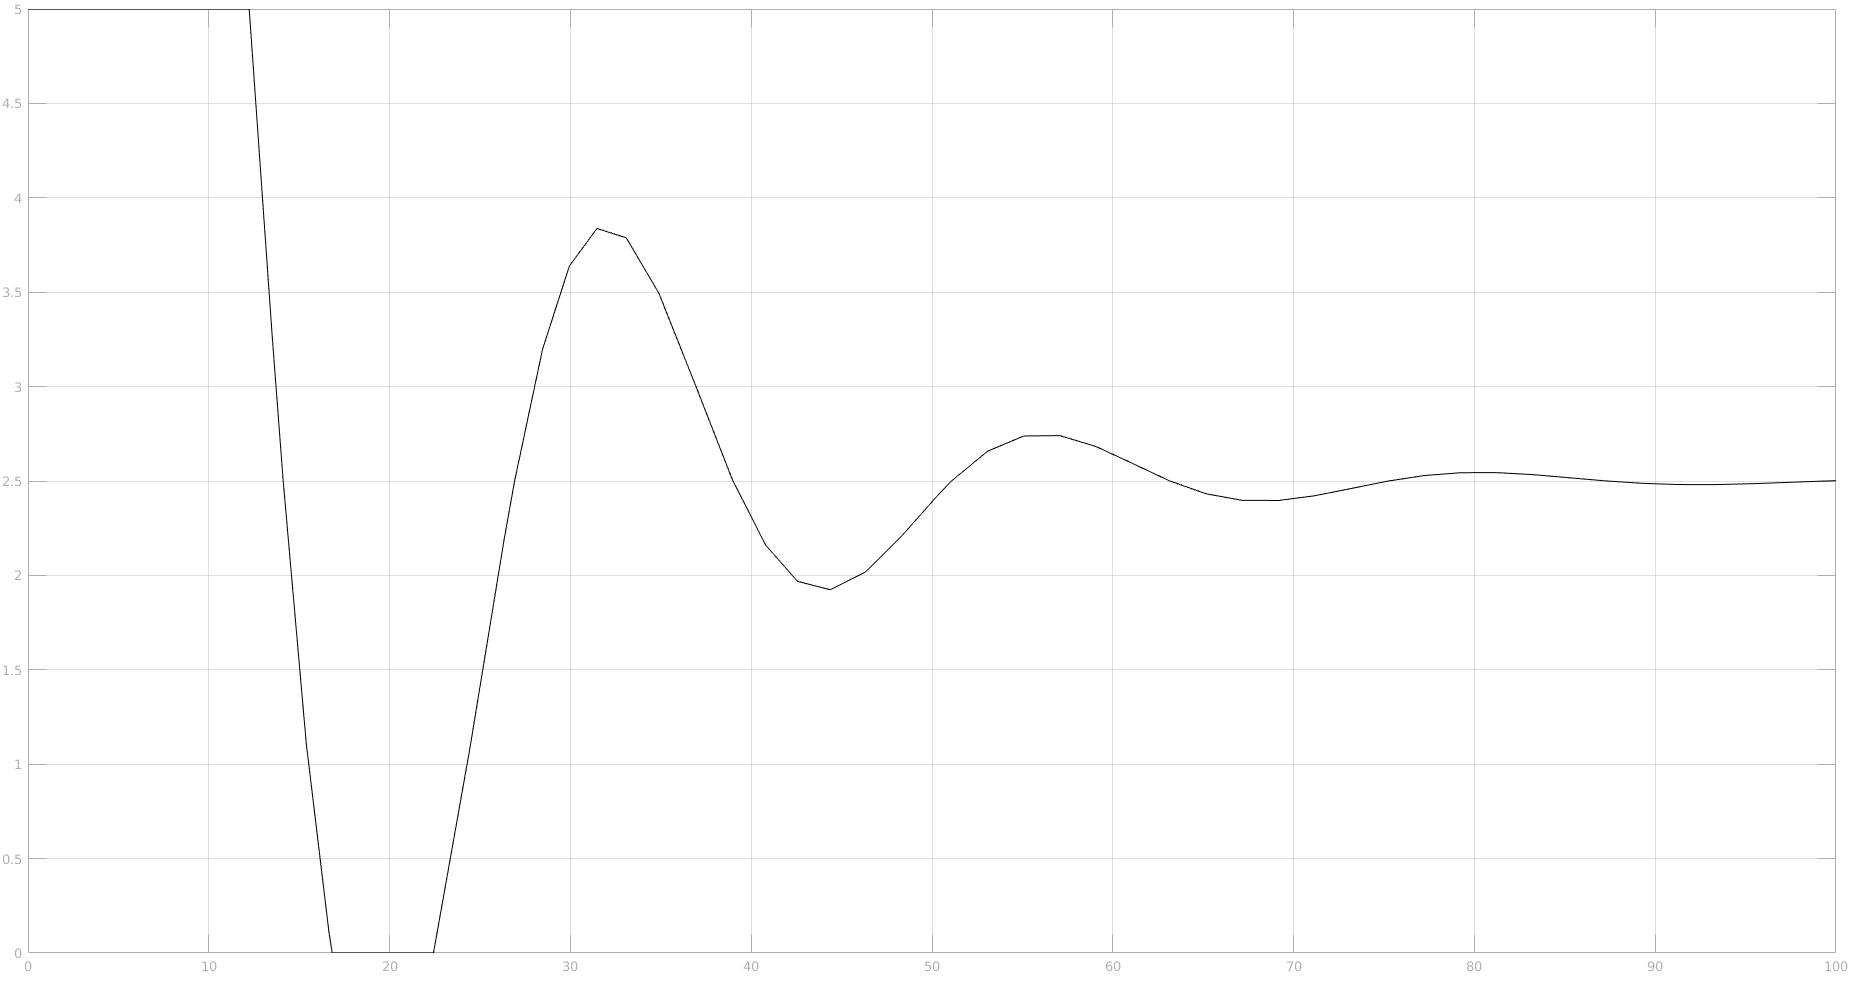
\includegraphics[width=1\linewidth]{Labo4_1_stuursignaal.jpg}
	\caption{tijdsverloop van het stuursignaal}
\end{figure}

\begin{figure}[!h]
	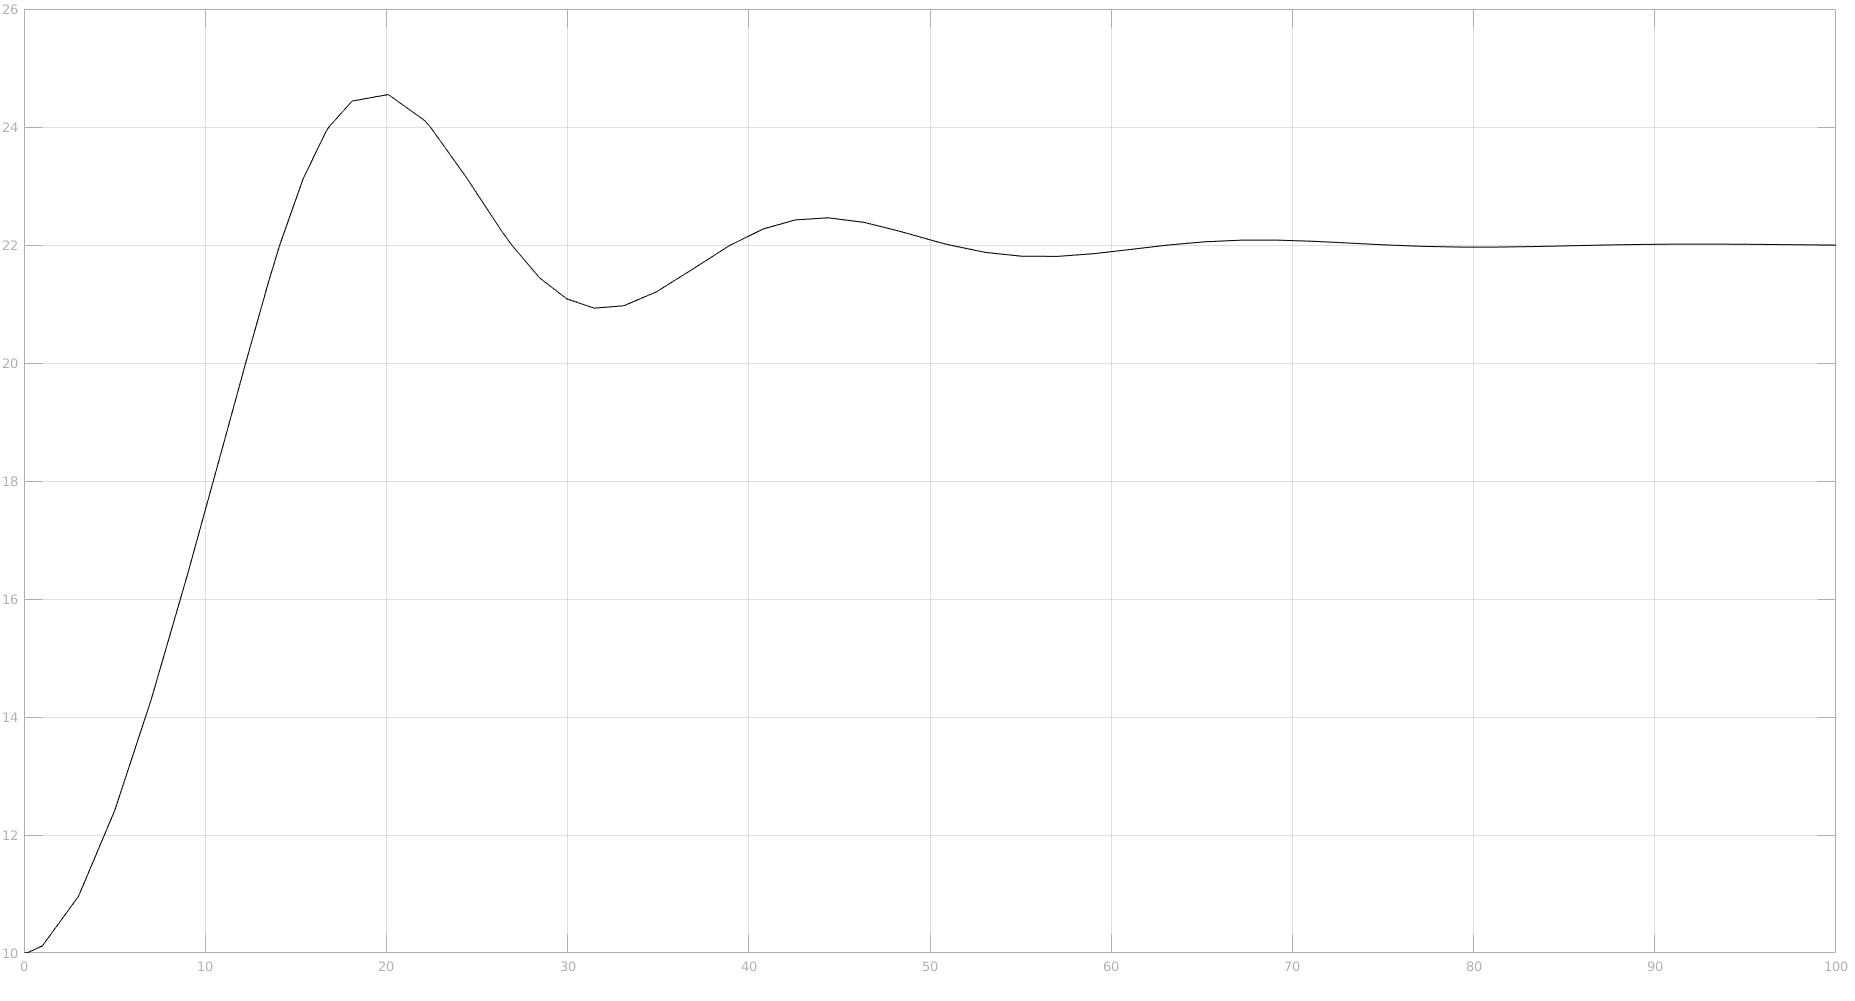
\includegraphics[width=1\linewidth]{Labo4_1_temperatuur.jpg}
	\caption{tijdsverloop van de temperatuur}
\end{figure}

In bovenstaande figuren zien we dat het stuursignaal op 2 momenten verzadigd is. Namelijk tussen 0 en 12 seconden, dan is het stuursignaal 5. En tussen 17 en 22 seconden, dan is het stuursignaal 0. We kunnen aan de hand van deze tijdsperiodes en het tijdsverloop zien wanneer het stuursignaal in verzadiging gaat. Dit is namelijk als de temperatuur lager is als $20^\circ$C en hoger als $24^\circ$C. Dit is niet toevallig $2^\circ$C hoger en lager als de ingestelde waarden. Dit is namelijk ingesteld in de regelaar. Dus als we als nieuwe instelwaarde $30^\circ$C zouden nemen, dan zal het stuursignaal in verzadiging gaan als de temperatuur lager is als $28^\circ$C en hoger is als $32^\circ$C.

\subsection{Voeg een scoop toe en observeer tegelijkertijd de signalen 'TE WARM', 'GOED' en 'TE KOUD'.}

\begin{figure}[!h]
	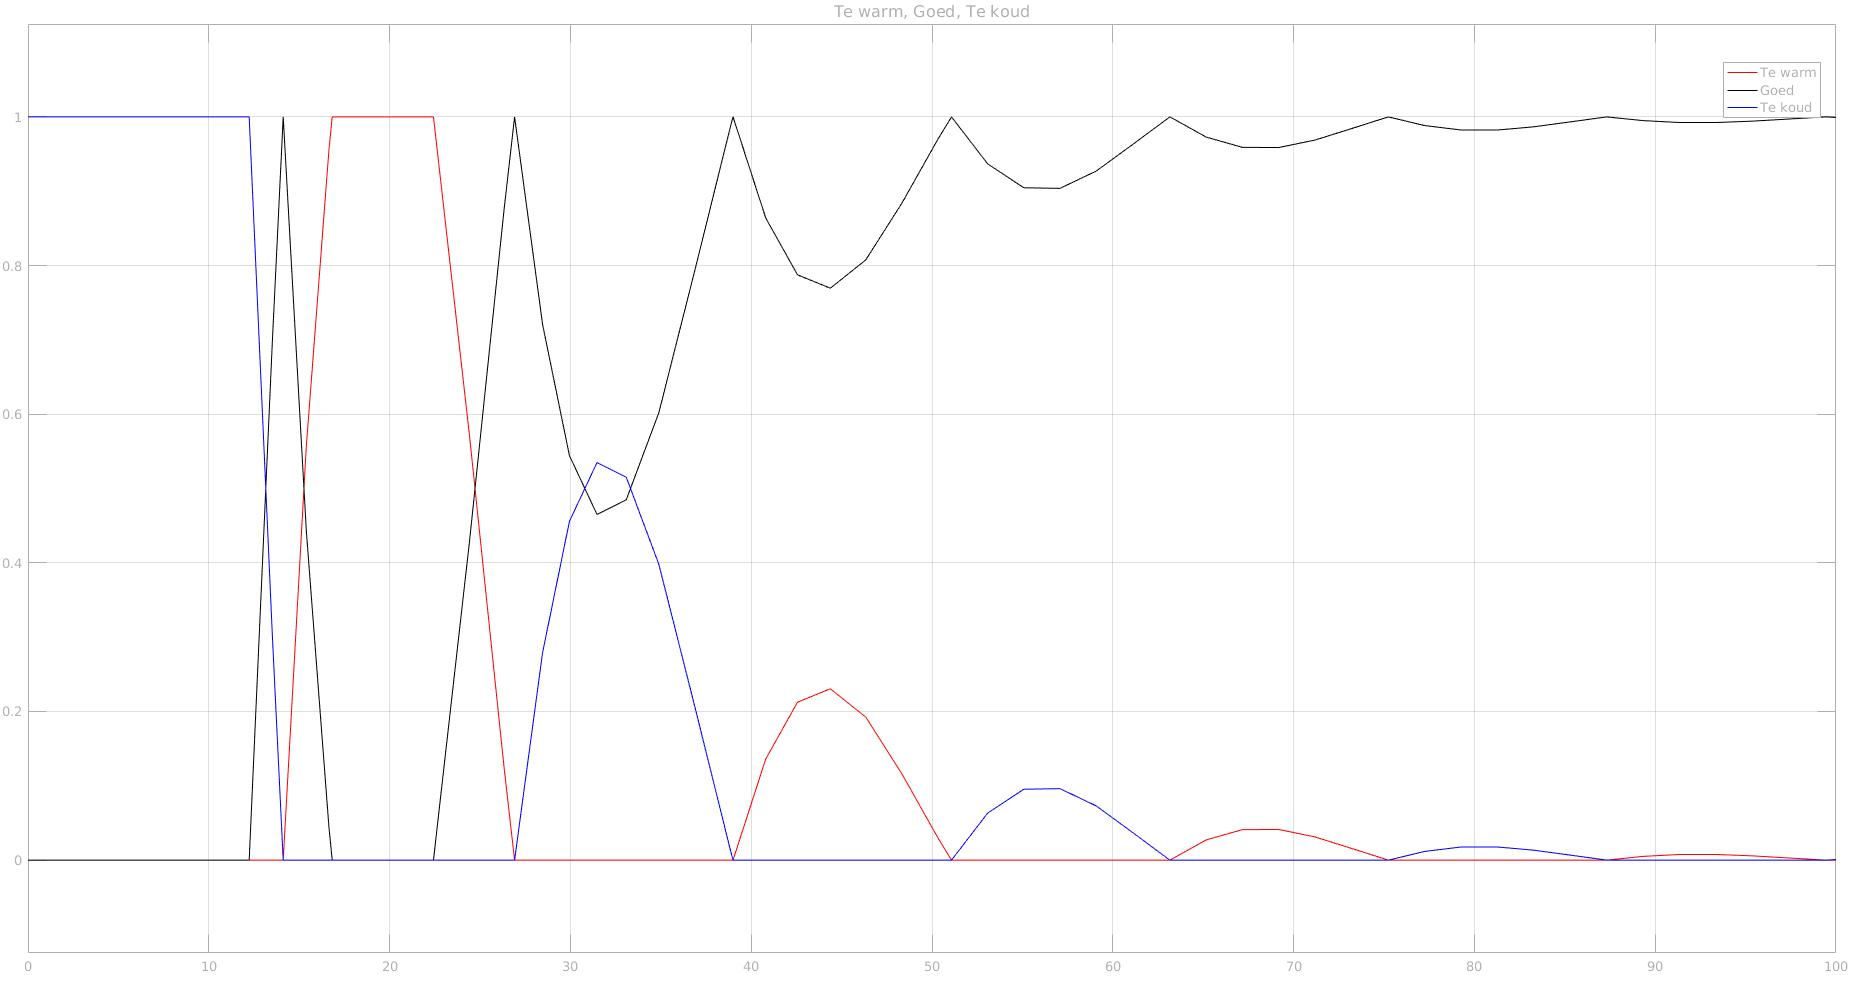
\includegraphics[width=1\linewidth]{Labo4_1_signals.jpg}
	\caption{tijdsverloop van de signalen 'TE WARM', 'GOED' en 'TE KOUD}
\end{figure}

\newpage

\subsection{Bekijk de ingangs/uitgangskarakteristiek van de fuzzy-regelaar m.b.v. het "test\_regelaar"-model. Dit model simuleert het verband tussen fout en stuursignaal. Voor de begininstelling komt dit overeen met een propotionele regelaar met verzadiging volgens figuur 8.2a.}


\begin{figure}[!h]
	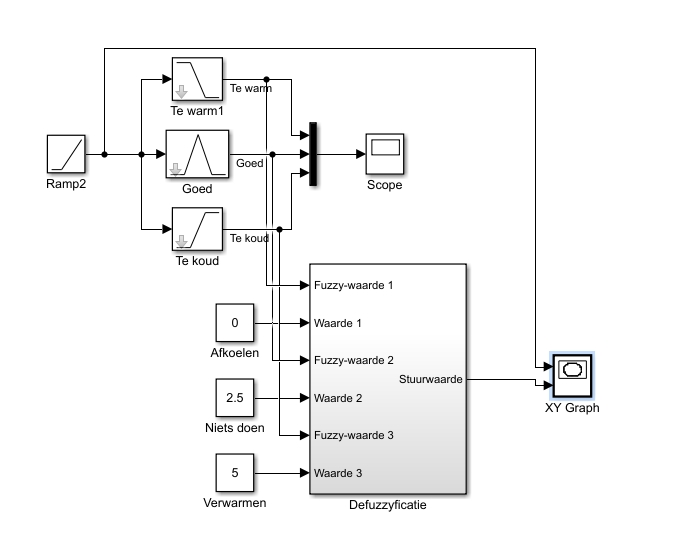
\includegraphics[width=1\linewidth]{Labo4_1_test_regelaar_screen.jpg}
	\caption{afbeelding van het gebruikte simulink schema}
\end{figure}

\begin{figure}[!h]
	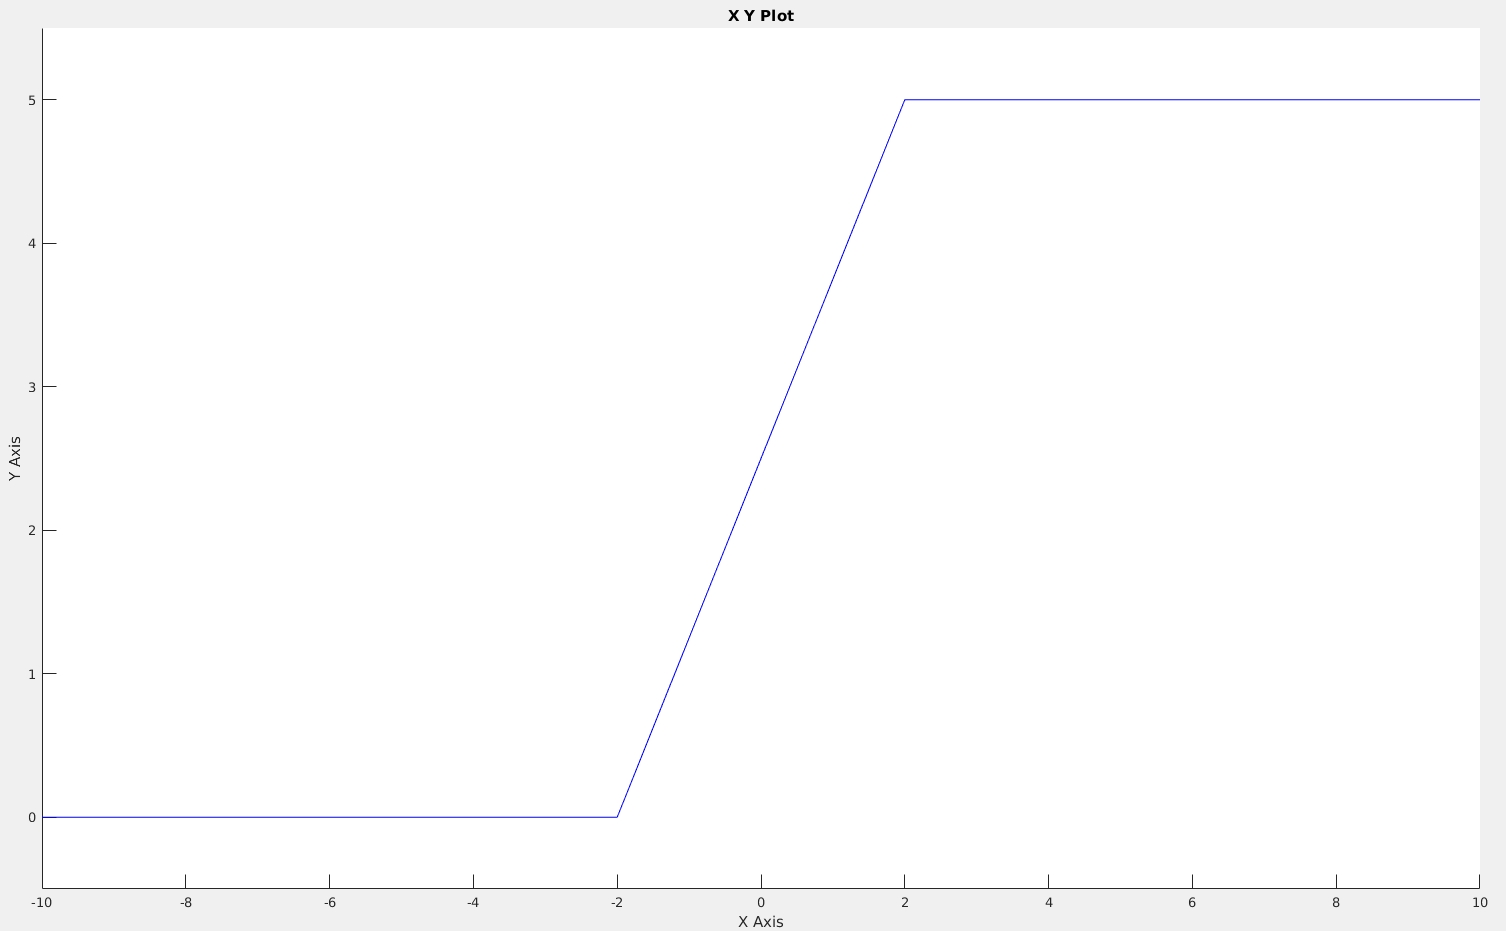
\includegraphics[width=1\linewidth]{Labo4_1_xy-plot.jpg}
	\caption{in/uit-karakteristiek}
	\label{fig:in/uit}
\end{figure}

\newpage

Op Figuur \ref{fig:in/uit} kunnen we zien dat de helling van de in/uit karakteristiek zich tussen -2 en 2 op de x-as bevind en zich 5 eenheden in de y-richting verplaatst. \\

$K\textsubscript{r} = \frac{5}{2-(-2)} = \frac{5}{4} = 1,25$ \\

\begin{figure}[!h]
	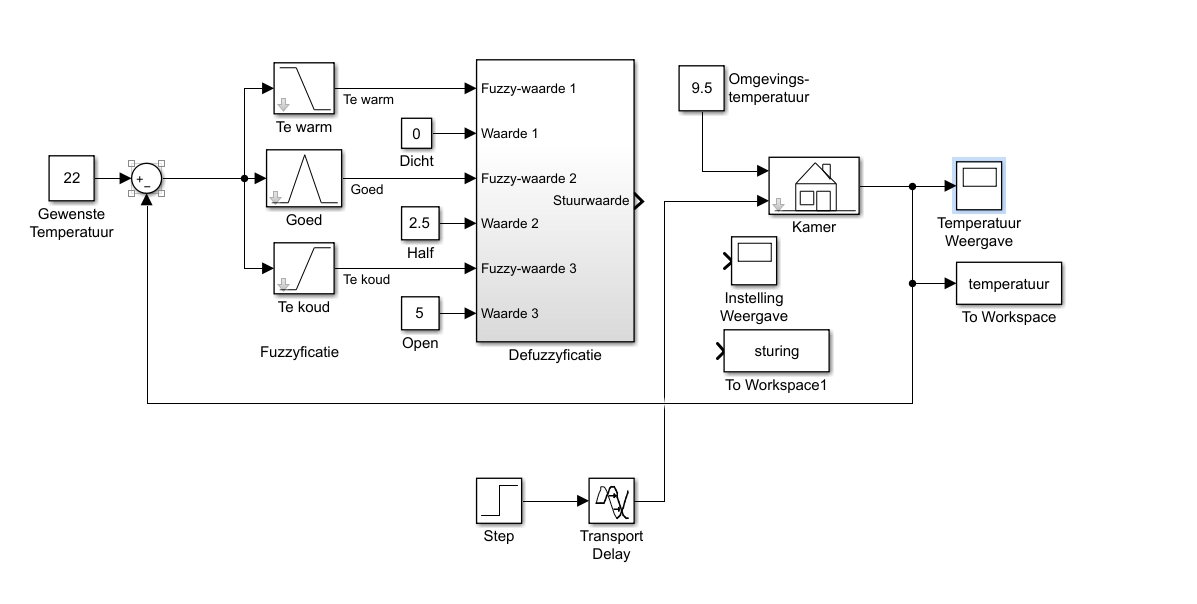
\includegraphics[width=1\linewidth]{Labo4_1_regellus_kamer_kp.jpg}
	\caption{afbeelding van de regellus met een step aan gelegd aan de kamer}
\end{figure}

\begin{figure}[!h]
	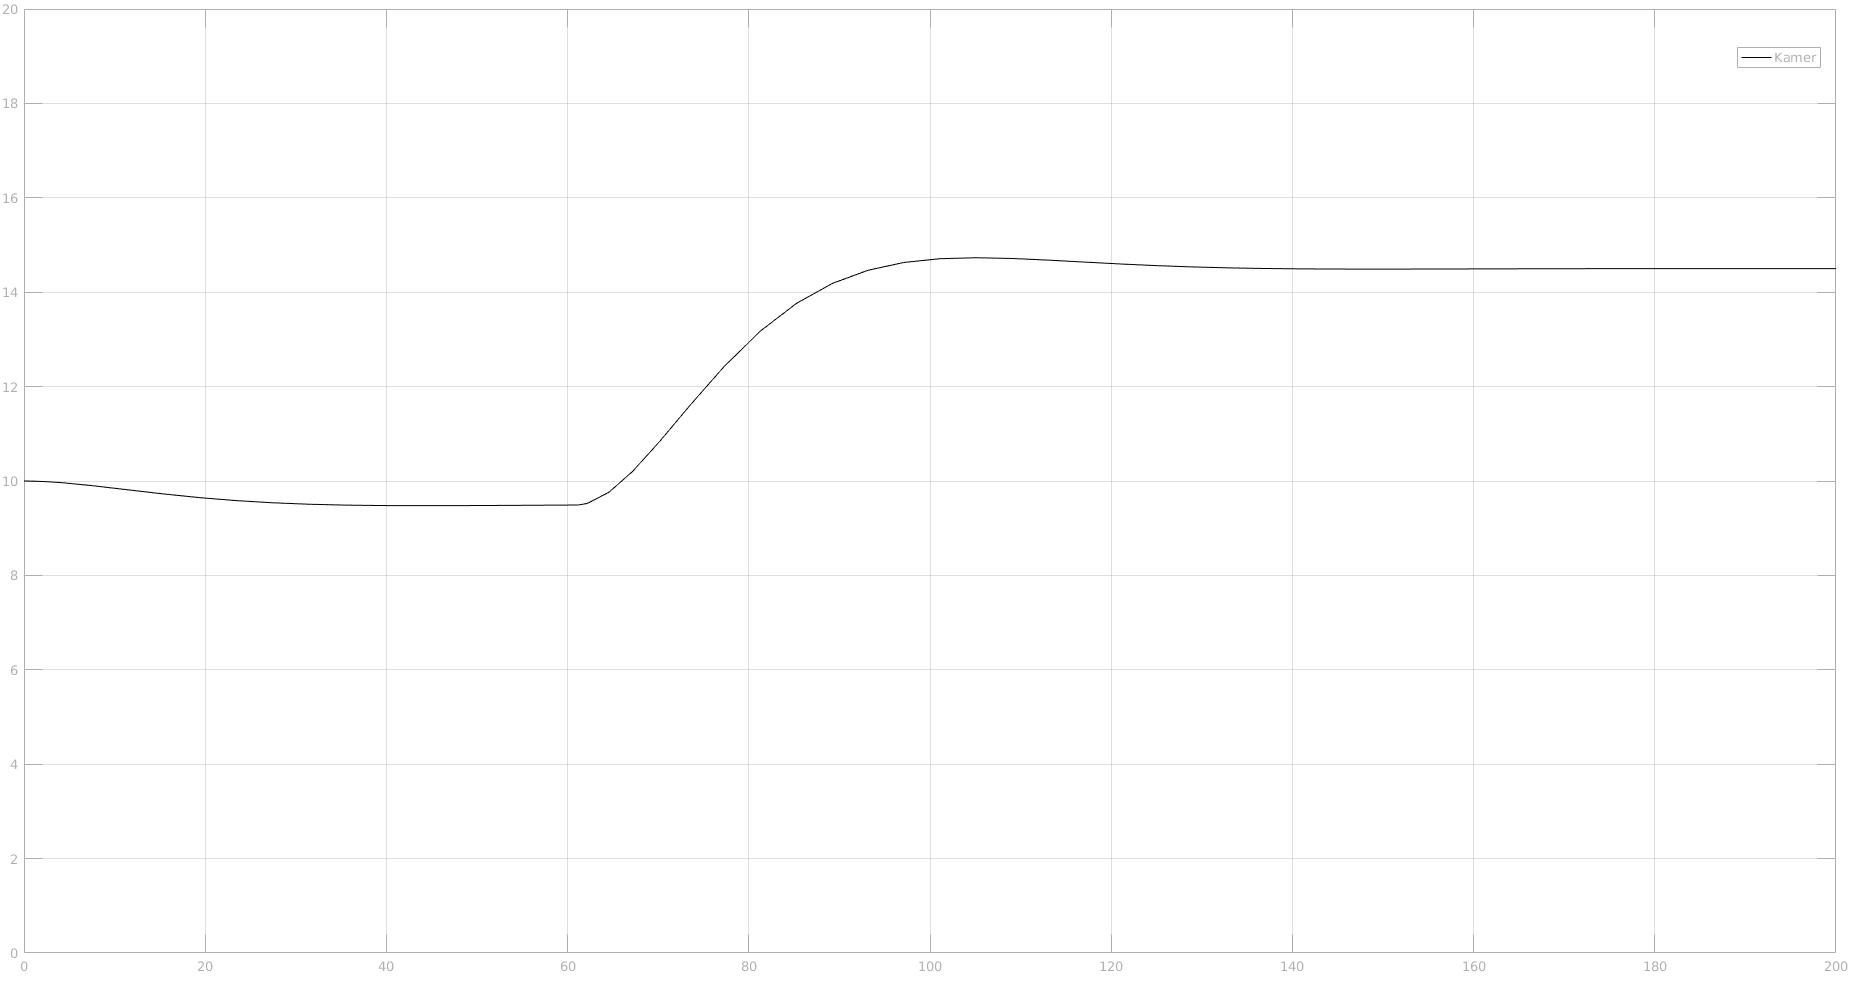
\includegraphics[width=1\linewidth]{Labo4_1_step_response_kamer.jpg}
	\caption{stap responsie van het kamer systeem}
\end{figure}

\newpage

De tijdsvertraging (aangezien het om een aangelegde stap gaat heeft die geen andere effecten dan een vertraging) die we hebben ingevoerd is om het systeem eerst te laten stabiliseren op $9,5^\circ$C voordat we de stap aanleggen. Dit is ook duidelijk te zien aan de stap responsie, de figuur gaat eerst tot 9,5 graden om dan stabiel te blijven tot aan 60s (de ingevoerde vertraging).\\
Na een zekere tijd zien we dat de figuur stabiliseert op $14,5^\circ$C. Dit wil zeggen dat we voor een aangelegde stap een stijging hebben van $14,5^\circ$C$ - 9,5^\circ$C$ = 5^\circ$C hebben. Dus K\textsubscript{p} heeft een waarde van 5. \\

De totale versterking is in dit geval $K = K\textsubscript{r} * K\textsubscript{p} = 6,25$. En hiermee kunnen we ook de standfout $\varepsilon\textsubscript{ss}$ berekenen. \\
$\varepsilon\textsubscript{ss} = \frac{1}{1+K} = \frac{1}{1+6,25} = 0,138 = 13,8\%$\\

Om de standfout te controleren hebben we de instelwaarde veranderd naar $30^\circ$. Dit omdat men bij $22^\circ$ geen standfout heeft. Hieruit kunnen we besluiten dat 22 het nulpunt is van het systeem. \\

\begin{figure}[!h]
	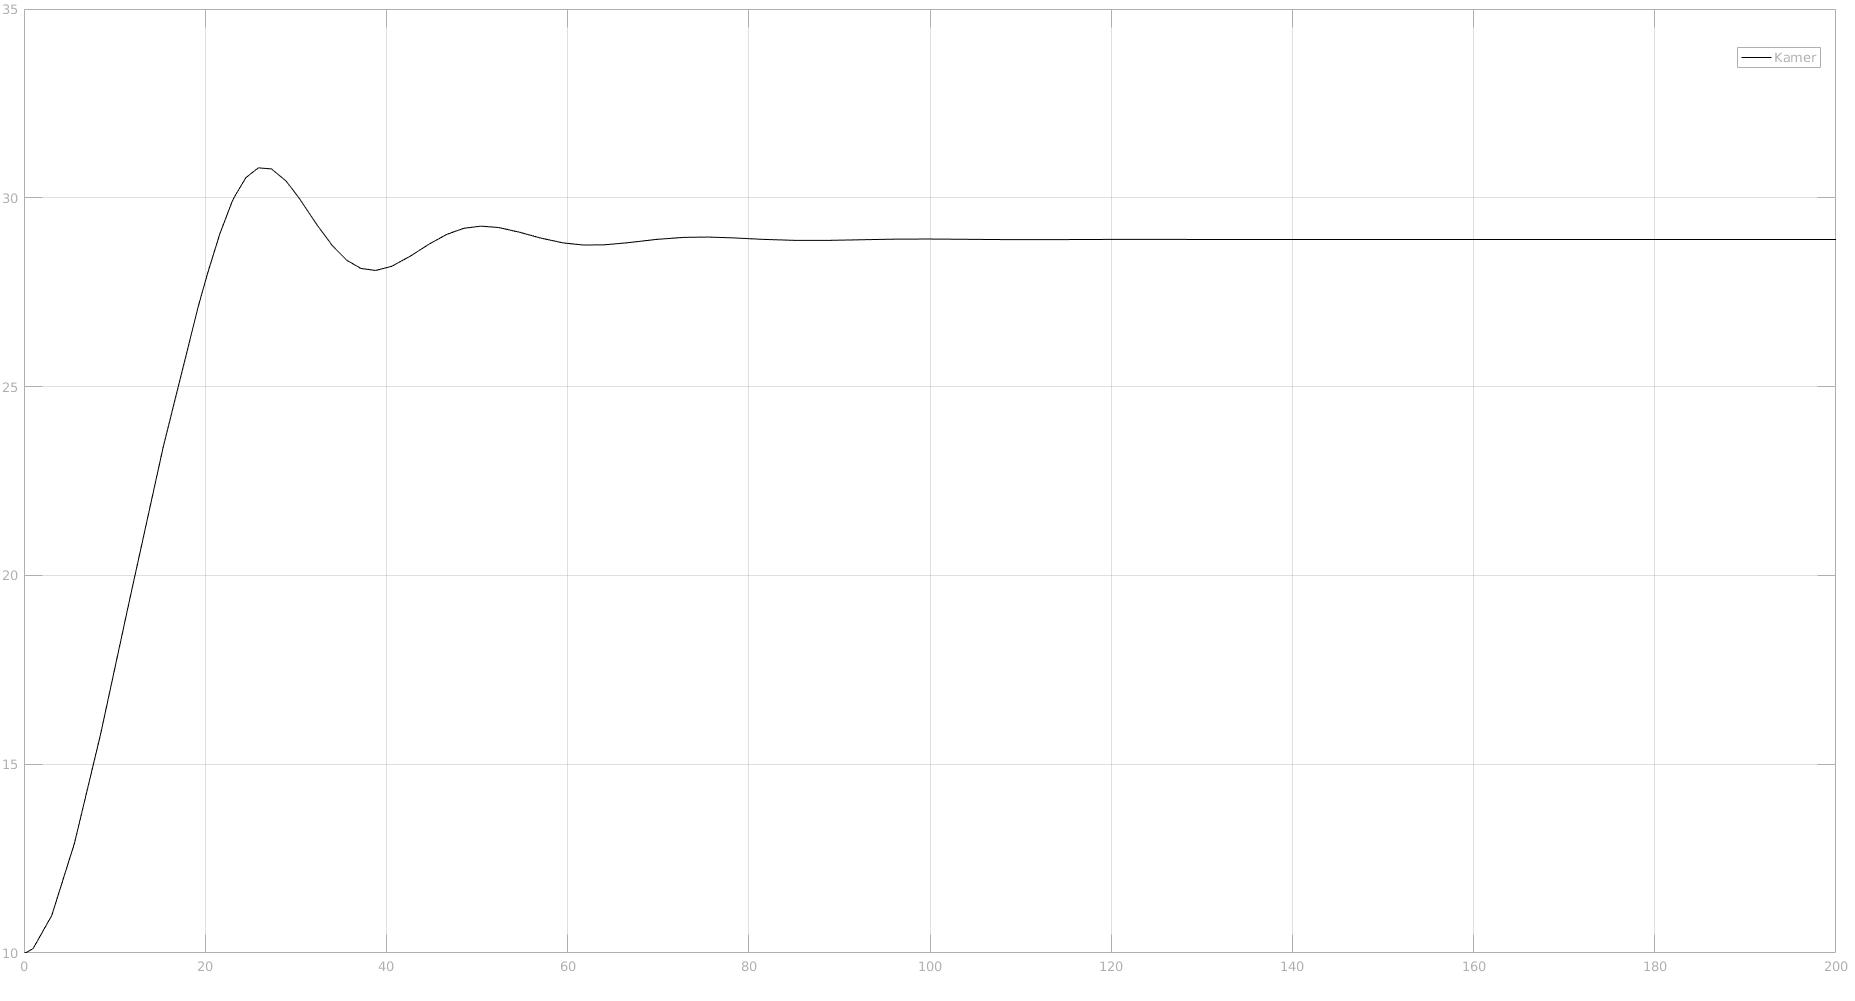
\includegraphics[width=1\linewidth]{Labo4_1_step_response_kamer_standfout.jpg}
	\caption {Het regelsysteem met een instelwaarde van $30^\circ$C}
	\label{fig:standfout}
\end{figure}

\newpage

In figuur \ref{fig:standfout} zien we de reactie van de kamer met het regelsysteem voor een instelwaarde van 30, doordat het systeem zich niet stabiliseert op deze 30 kunnen we besluiten dat er een standfout heerst. Het systeem stabiliseert zich dus niet op 30 maar op 28,9.\\
$\varepsilon\textsubscript{ss} = \frac{30-28,9}{30-22} = 0,138 = 13,8\%$\\
Dus ook via een experimentele methode komen we uit op een standfout van 13,8\%.

\subsection{Pas de fuzzyficatiecurven aan zodanig dat de ingangs/uitgangskarakteristiek van de regelaar overeenstemt met figuur 1b of 1c}

Om figuur 1b te bekomen doen we de volgenden instellingen: 
\begin{table}[!h]
\centering
\resizebox{\columnwidth}{!}{
	\begin{tabular}{p{0.4\linewidth} p{0.6\linewidth}}
	TE WARM & -4 tot 0\\
	GOED & -4 tot 2\\
	TE KOUD & 0 tot 2\\
	\end{tabular}
}
\end{table}

\begin{figure}[!h]
	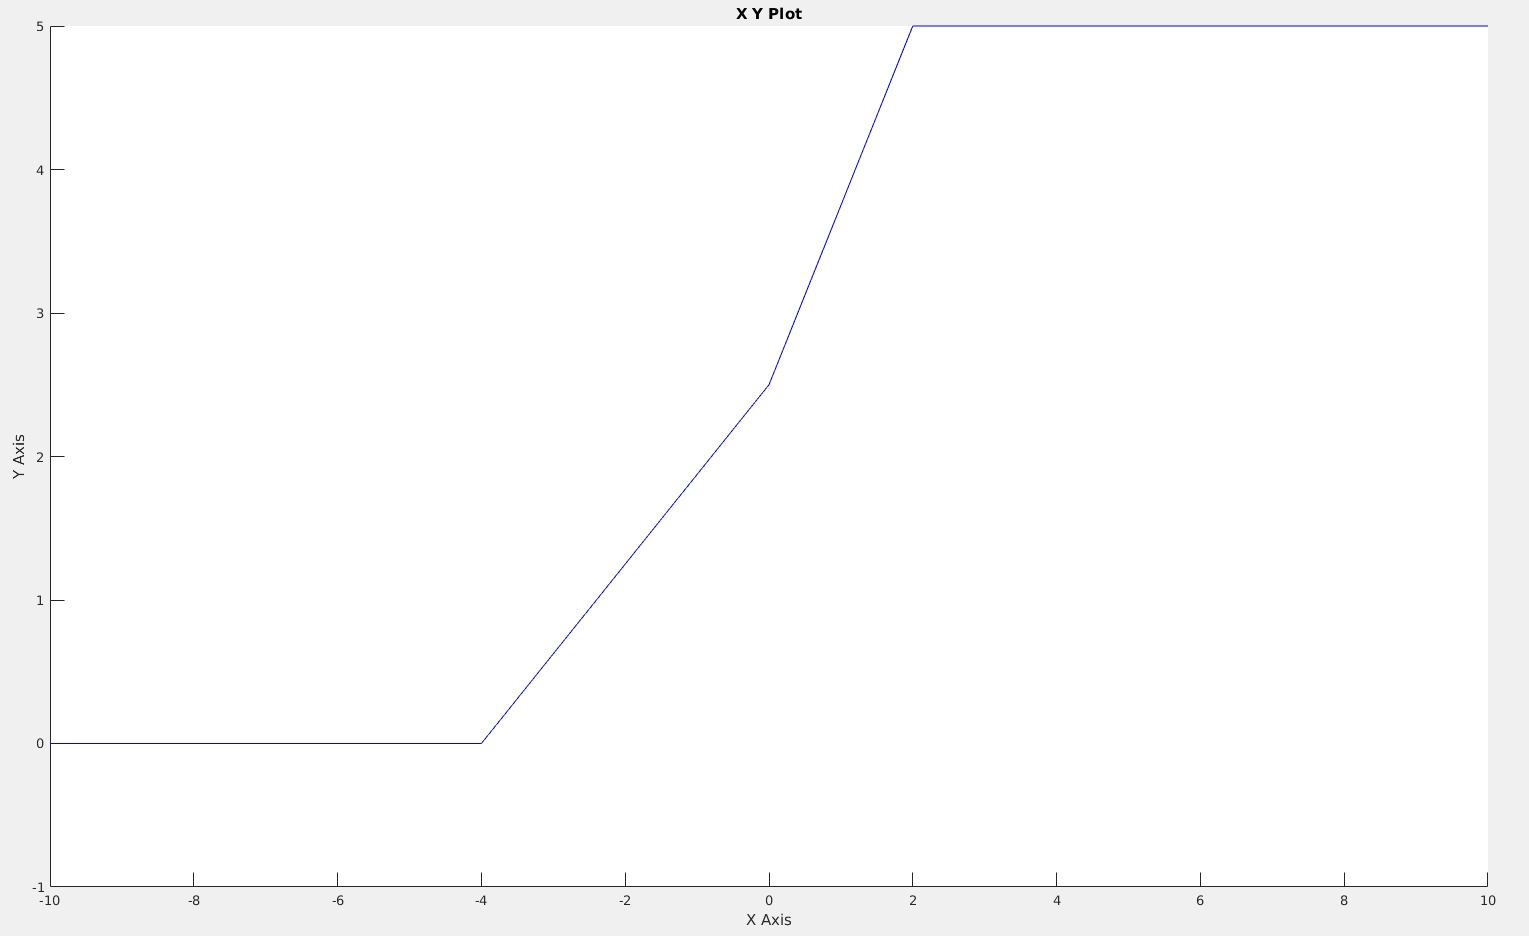
\includegraphics[width=0.9\linewidth]{Labo4_1_fig1b.jpg}
	\caption{fig1b}
\end{figure}

\newpage

\begin{table}[!h]
\centering
\resizebox{\columnwidth}{!}{
	\begin{tabular}{p{0.4\linewidth} p{0.6\linewidth}}
	TE WARM & -1 tot 0\\
	GOED & -4 tot 4\\
	TE KOUD & 0 tot 1\\
	\end{tabular}
}
\end{table}

\begin{figure}[!h]
	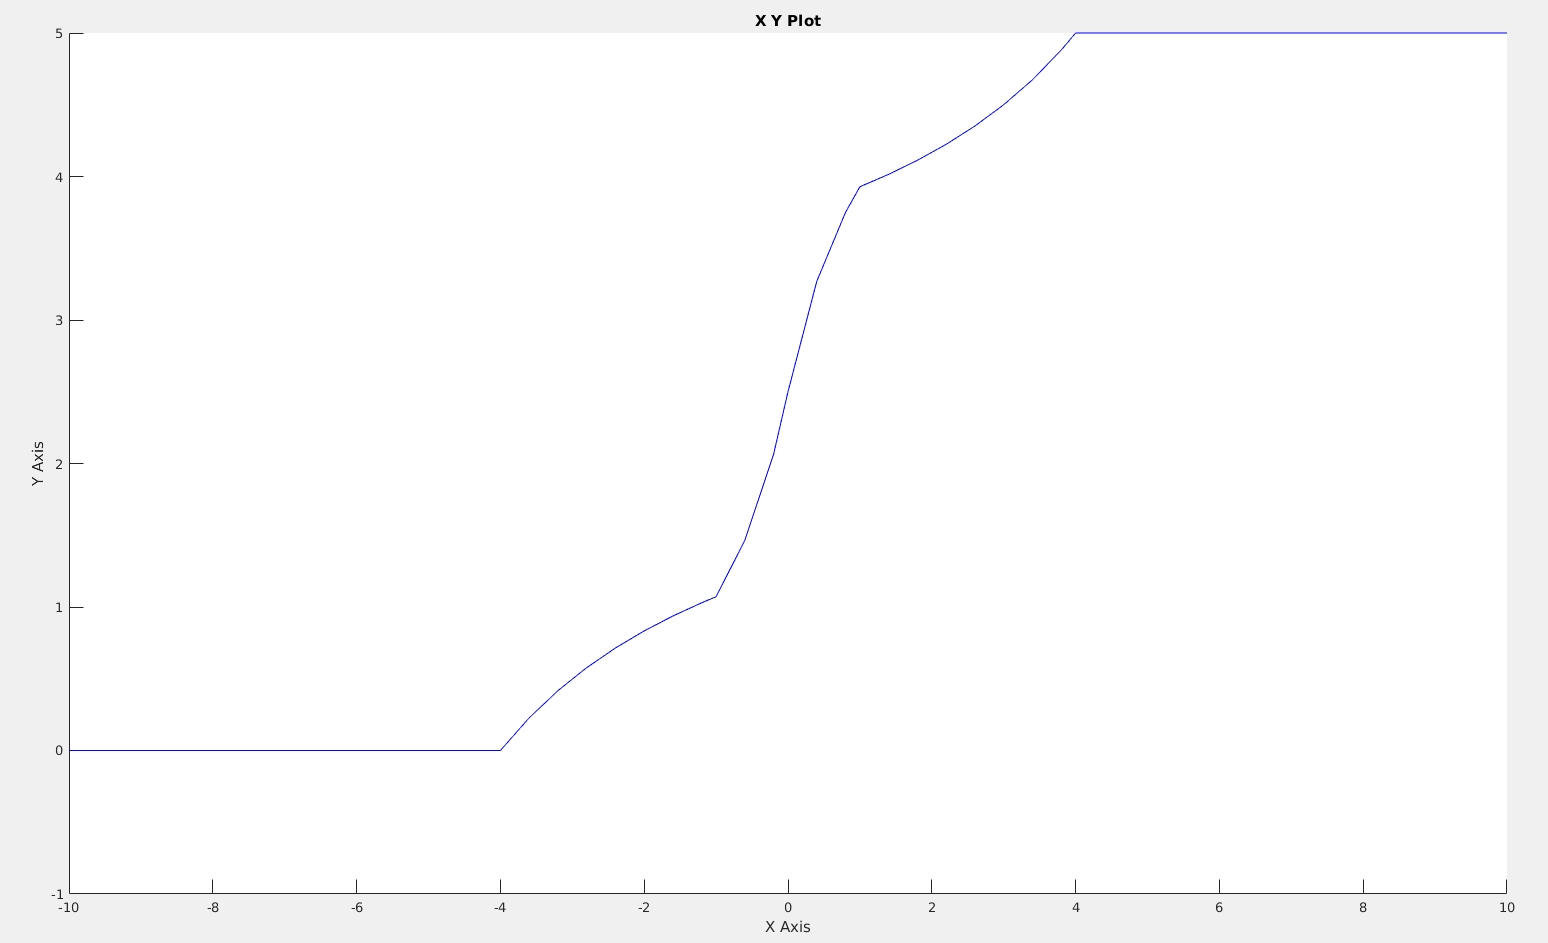
\includegraphics[width=0.9\linewidth]{Labo4_1_fig1c.jpg}
	\caption{fig1c}
\end{figure}

\newpage

\begin{table}[!h]
\centering
\resizebox{\columnwidth}{!}{
	\begin{tabular}{p{0.4\linewidth} p{0.6\linewidth}}
	TE WARM & -4 tot -1\\
	GOED & -1 tot 1\\
	TE KOUD & 1 tot 4\\
	\end{tabular}
}
\end{table}

\begin{figure}[!h]
	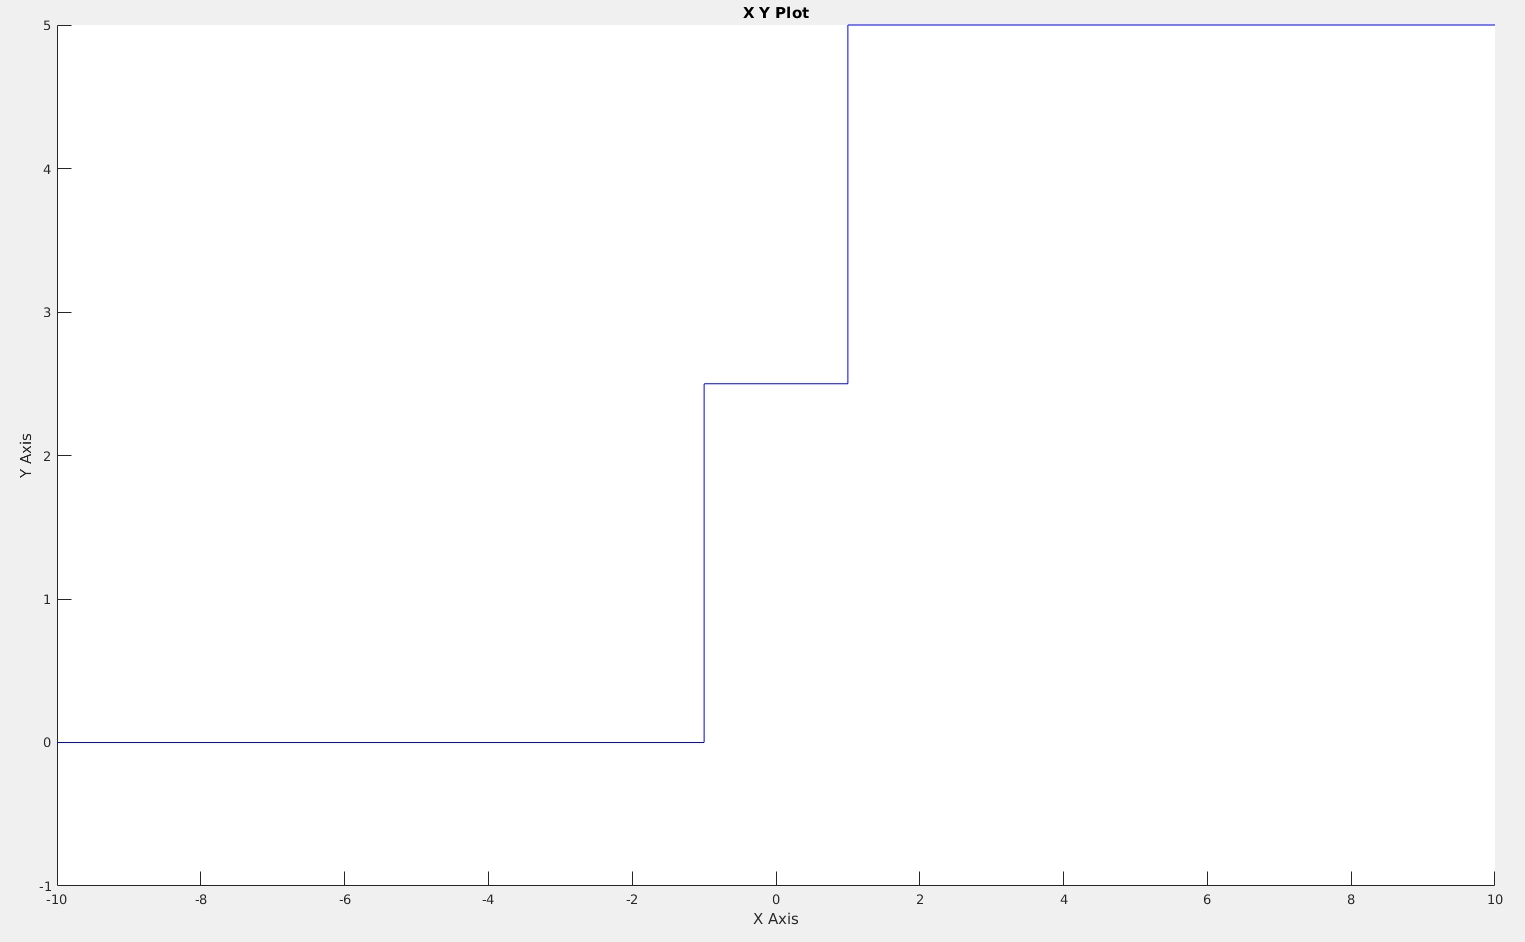
\includegraphics[width=1\linewidth]{Labo4_1_rechte.jpg}
	\caption{3 rechte lijnstukken}
\end{figure}

\newpage

\section{aanpassingen}

Hoe moeten we het regelschema aanpassen en de fuzzyregels aanpassen om de standfout te elimineren? \\

Een standfout elimineren is vrij simpel. Dit kunnen we doen door ergens in het schema een zuiver integrator bij te plaatsen. Deze zou de standfout te niet moeten doen.

\begin{figure}[!h]
	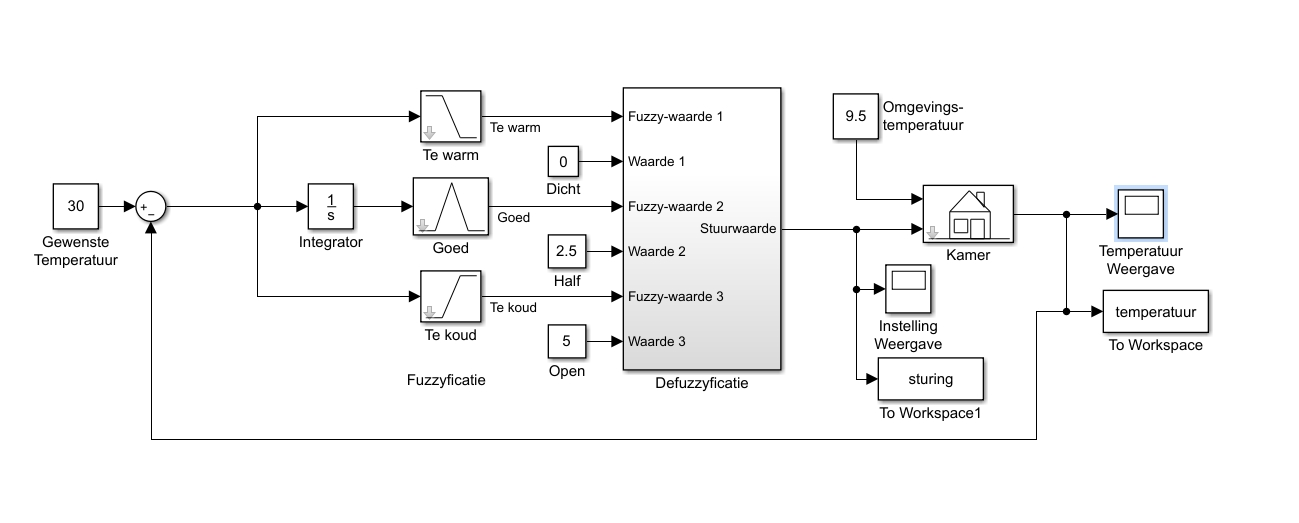
\includegraphics[width=1\linewidth]{Labo4_1_system_no_error.jpg}
	\caption{Schema van het systeem met extra integrator}
\end{figure}

\begin{figure}[!h]
	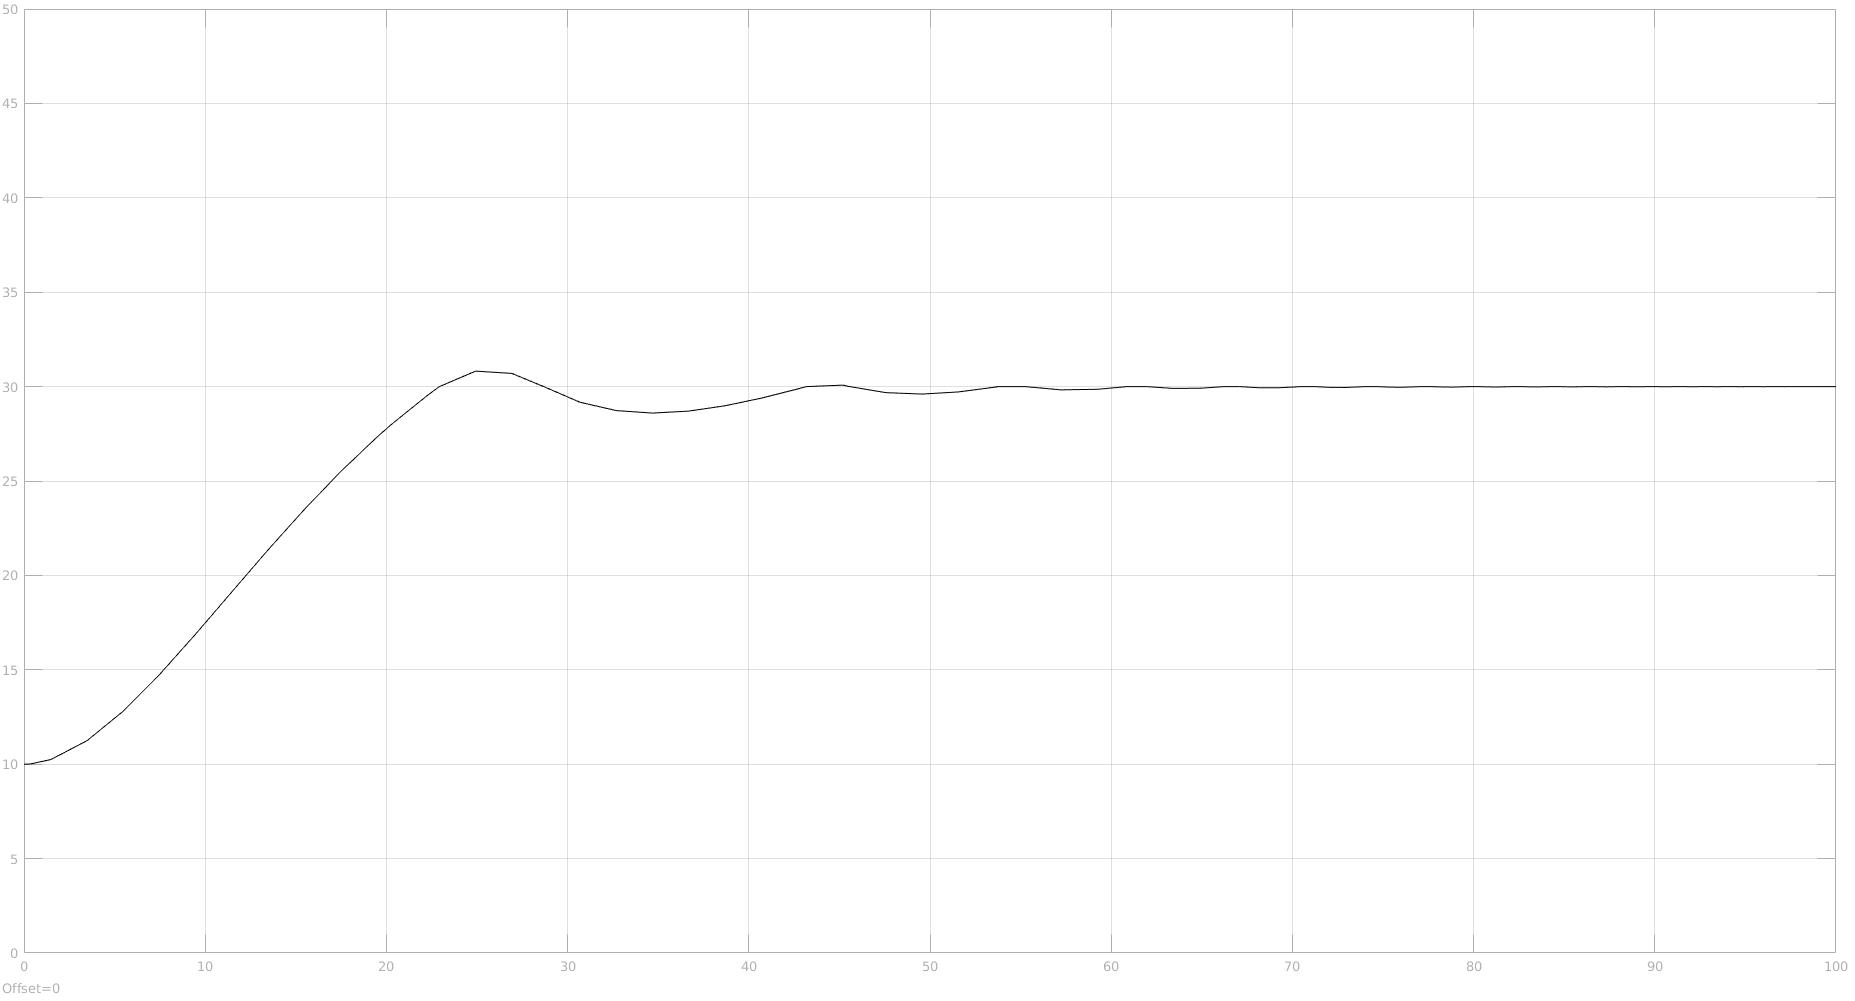
\includegraphics[width=1\linewidth]{Labo4_1_temperatuur_no_stand_fout.jpg}
	\caption{De reactie van het regelsysteem met integrator dus zonder standfout}
\end{figure}

\end{document}